\documentclass[pdf, ignorenonframetext]{beamer}
\mode<presentation>{}
\usepackage{libertine}
\usepackage[sharp]{easylist}


% NB: this is PANTONE "Blue Sapphire" 18-4231
\definecolor{ChristoBlueSapphire}{RGB}{18, 97, 128}
\setbeamercolor{palette tertiary}  {bg=ChristoBlueSapphire,fg=white}
\setbeamercolor{palette quaternary}{fg=black,bg=white}
\setbeamercolor{structure}{fg=ChristoBlueSapphire}
\setbeamercolor{titlelike}         {bg=ChristoBlueSapphire,fg=white}
\setbeamercolor{frametitle}        {bg=ChristoBlueSapphire!10,fg=ChristoBlueSapphire}

\setbeamertemplate{navigation symbols}{}

\begin{document}

\begin{frame}[plain, fragile, t]{A Browser-based MEI Editor (meix.js)}
\vspace{0.37cm}
	\begin{columns}
	\scriptsize
		\begin{column}{0.2\textwidth}
	    Andrew Horwitz \\(ahwitz@gmail.com)
	    \end{column}
	    \begin{column}{0.35\textwidth}
	    Andrew Hankinson \\(andrew.hankinson@mail.mcgill.ca)
	    \end{column}
	    \begin{column}{0.2\textwidth}
	    Ichiro Fujinaga \\(ich@music.mcgill.ca)
	    \end{column}
	\end{columns}

	\vspace{\baselineskip}
	\vspace{-0.5cm}
	\tiny
	\begin{center}
	Distributed Digital Music Archives and Libraries Lab, CIRMMT, Schulich School of Music, McGill University
	\end{center}

	\vspace{-1cm}

	\begin{block}{}
		\scriptsize
        \begin{columns}
        \begin{column}{\textwidth}
            \begin{block}{}
                \centering
                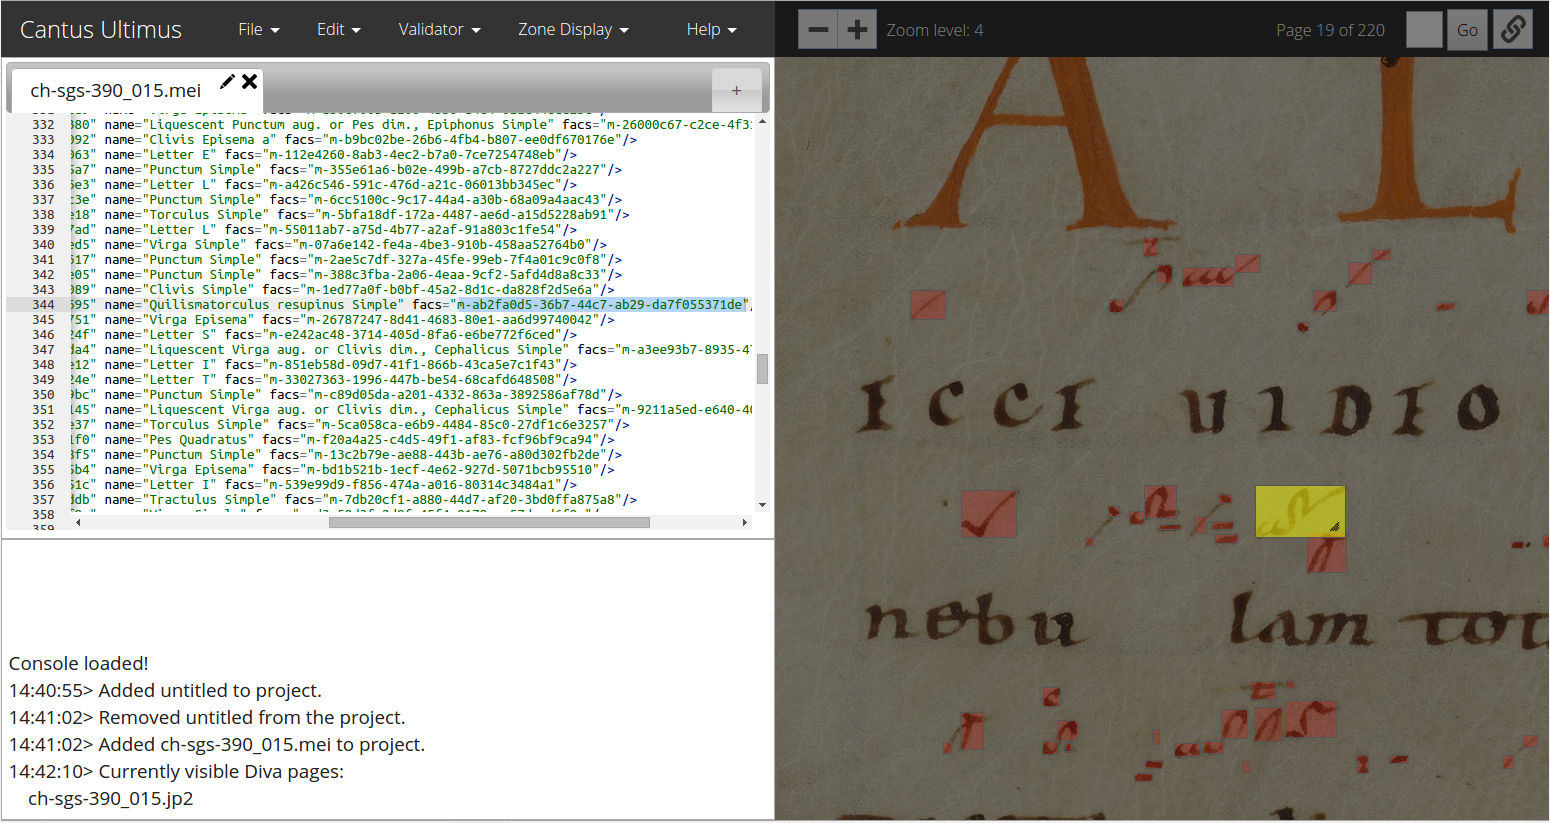
\includegraphics[scale=0.15]{mei_editor_diva}
	            \begin{block}{St. Gallen}
	    			\vspace{.5\baselineskip}
	                http://dev-cantus.simssa.ca/editor/
	    			\vspace{\baselineskip}
	    
	           		meix.js synchronizes with a Diva.js document viewer pane for editing MEI representations of music manuscripts.
	            \end{block}
            \end{block}
        \end{column}
        \end{columns}
    \end{block}
\end{frame}

\begin{frame}[plain, fragile, t]{A Browser-based MEI Editor (meix.js)}
\vspace{0.37cm}
	\begin{columns}
	\scriptsize
		\begin{column}{0.2\textwidth}
	    Andrew Horwitz \\(ahwitz@gmail.com)
	    \end{column}
	    \begin{column}{0.35\textwidth}
	    Andrew Hankinson \\(andrew.hankinson@mail.mcgill.ca)
	    \end{column}
	    \begin{column}{0.2\textwidth}
	    Ichiro Fujinaga \\(ich@music.mcgill.ca)
	    \end{column}
	\end{columns}

	\vspace{\baselineskip}
	\vspace{-0.5cm}
	\tiny
	\begin{center}
	Distributed Digital Music Archives and Libraries Lab, CIRMMT, Schulich School of Music, McGill University
	\end{center}


	\vspace{-1cm}

	\begin{block}{}
		\scriptsize
        \begin{columns}
        \begin{column}{\textwidth}
            \begin{block}{}
                \centering
                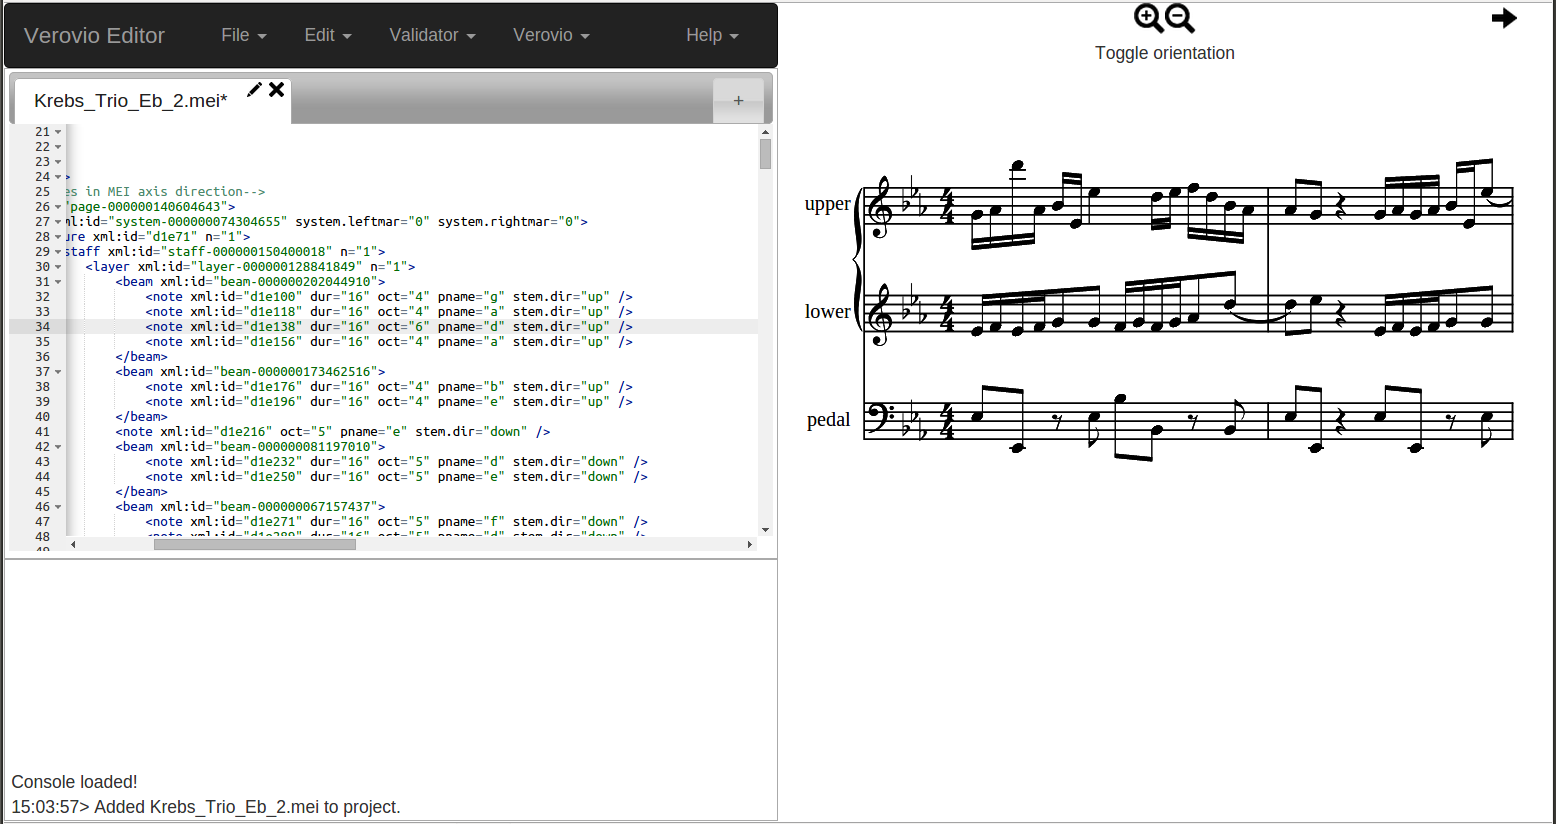
\includegraphics[scale=0.15]{mei_editor_verovio}

	            \begin{block}{Verovio}
	    			\vspace{.5\baselineskip}
	                http://dev.simssa.ca/veditor/
	    			\vspace{\baselineskip}

	    			meix.js synchronizes with a Verovio-generated paginated score with drag-and-drop editing functionality.
	            \end{block}
            \end{block}
        \end{column}
        \end{columns}
    \end{block}
\end{frame}

\end{document}